\section{Application to Compressive Sensing}
\label{ch:cs}
\subsection{Introduction}
% SPI definition and main stages
Single-pixel imaging (SPI) is a relatively recent imaging technique that replaces the classic two dimensional sensor array with a single photodetector~\cite{bian2018experimental}. An SPI camera modulates the incoming light from a scene using a light modulator, such as a diffuser~\cite{guo2016multilayer} or a digital micro-mirror device (DMD)~\cite{pittman1995optical, sampsell1993overview}, and focuses the resulting correlated light patterns onto a photodiode. The configuration of the modulator and the recorded intensity of light are then processed to reconstruct an image of the target scene.

% advantages of SPI
SPI owes its popularity to multiple advantages it achieves over traditional imaging approaches that employ 2D sensor arrays. First, since all reflected light is focused onto a single detector, SPI has better sensitivity under dim lighting conditions and enjoys a broader spectral range\cite{Edgar2019}. Second, SPI moves the cost of acquisition and processing from the encoding/compression stage to the decoding/reconstruction stage. For example, a DMD array orients its mirrors to reflect light either towards the detector (+1) or away from it (0). Importantly, these orientations do not depend on the scene that is being acquired to ensure proper reconstruction: \cite{baraniuk2008simple}~showed that DMD patterns can be drawn as independent identically distributed (i.i.d.) samples from a uniform Bernoulli distribution. In contrast, sample-then-compress approaches\cite{skodras2001jpeg} require an expensive projection of multiple single-pixel snapshots onto a chosen basis, such as Fourier or top-K singular vectors, during their encoding step. Doing the heavy-lifting job during decoding is often preferred in applications where sensors have to be small and low-power, whereas decoding happens offline on high-performance computers. The simplicity of encoding keeps the computational requirements of SPI sensors (and thus their price) low, inviting their application in multispectral imaging \cite{bian2016multispectral,li2017efficient}, optical encryption~\cite{chen2013ghost}, remote sensing~\cite{zhao2012ghost}, object tracking~\cite{li2014ghost}, and many other fields~\cite{sun20133d,zhang2010correlated,cheng2009ghost}.

% introducing CS
Compressive Sensing (CS)~\cite{donoho2006compressed, candes2006compressive, baraniuk2014introduction, baraniuk2008simple} emerged in the mid-2000s as an alternative signal acquisition regime to classical Shannon-Nyquist sampling. In the classical regime, a band-limited signal is sampled at $N$ specific points in time (and/or space) so that the signal can be reconstructed from the acquired samples using a simple Sinc interpolation. Compressive sensing, on the other hand, proposes to acquire the signal using a small number of inner products between the signal and general non-adaptive sampling vectors. If the signal to be acquired has a $K$-sparse, or more generally, parsimonious, representation some transform domain, then the signal can be guaranteed to be recovered using as few as $\mathcal{O}(K\log(N/K))$ non-adaptive measurements, which is much smaller than the $N$ samples that are required by sample-then-compress approaches such as JPEG and JPEG-2000~\cite{skodras2001jpeg}. The development of compressive sensing theory and efficient reconstruction algorithms has further promoted the deployment of this technique in SPI~\cite{duarte2008single}.

% Compressive Sensing (CS) is an approach to SPI which assumes that a signal is spare in a certain basis. Under this assumption a small collection of non-adaptive linear measurements can contain enough information for reconstructing the signal~\cite{duarte2008single, candes2006compressive}. Namely, when an original signal made of $N$ pixels has a $K$-sparse representation in a certain basis, the basis coefficients can be recovered using only $\mathcal{O}(K\log(N/K))$ which is much smaller than $N$ required by sample-then-compress approaches such as JPEG and JPEG-2000~\cite{skodras2001jpeg}.

% Recent progress on deep SPI
Because each CS measurement contains highly-compressed information about the observed frame, one needs to sample a large number of such measurements. Thus, many recent works propose approaches to reduce the number of required samples per frame (SPF). These approaches can be roughly grouped into two buckets: signal-dependent control of the mirrors and more sophisticated reconstruction techniques. The former ensures that each single-pixel measurement contains as much information as possible by focusing the mirrors on the selected regions of the frame~\cite{zhang2017fast,sun2017russian,xu20181000}. Although highly effective, such an approach cannot be applied to monitoring scenes that don't have a ``main zone'' where the information acquisition could be focused. For example, a camera monitoring a gas tank for leaks can not have a mask that works well for leaks appearing only in the middle of the scene. The second group of approaches focuses on creating more efficient optimization algorithms for the decoding step~\cite{katz2009compressive}. It includes non-iterative algorithms such as differential ghost imaging (DGI) \cite{gong2010method}, as well as iterative methods such as total variation (TV)~\cite{suo2016signal} regularization. Notably, recent approaches adopted deep learning (DL) for SPI reconstruction. These approaches showed that using deep neural networks can dramatically reduce sampling ratio and offer near-real-time performance \cite{lyu2017deep,higham2018deep,wang2019learning,wang2022single}. However, most of these methods use multiple samples for single-frame reconstruction and do not yield satisfactory reconstruction of multiple sequential frames when the number of samples per frame is small, even if the total number of samples is large, as we show below.

% Our place among CS literature
Our work aims to bridge this gap. It falls into the second group of decoding-centered approaches which aid CS reconstruction with deep learning. In particular, we show how a Reduced-Order Model (ROM) can be used to regularize CS reconstruction of a video of a physical phenomenon, even if all the measurements are taken at different moments in time. We achieve that by pre-training a ROM to compress simulations into a latent space and calculate the system's evolution there using neural ordinary differential equations (neural ODEs). At the time of reconstruction, we recover a trajectory in the latent space which yields compressing sensing measurements that match what the detector recorded when projected to the observable space. Effectively, we solve an ODE-regularized CS reconstruction in an efficient way using the adjoint-sensitivity method to obtain necessary derivatives~\cite{chen2018neuralode}. Such ODE-based regularization serves as a strong induced bias and reduces the number of samples per frame required for a successful reconstruction. In fact, our method requires fewer samples per frame than the current state-of-the-art methods. We introduce the methodology in Section~\ref{sec:cs_methods} and study its performance on two examples: Burger's equation and Kolmogorov flow.

\subsection{Methods}
\label{sec:cs_methods}
\begin{figure}
    \centering
    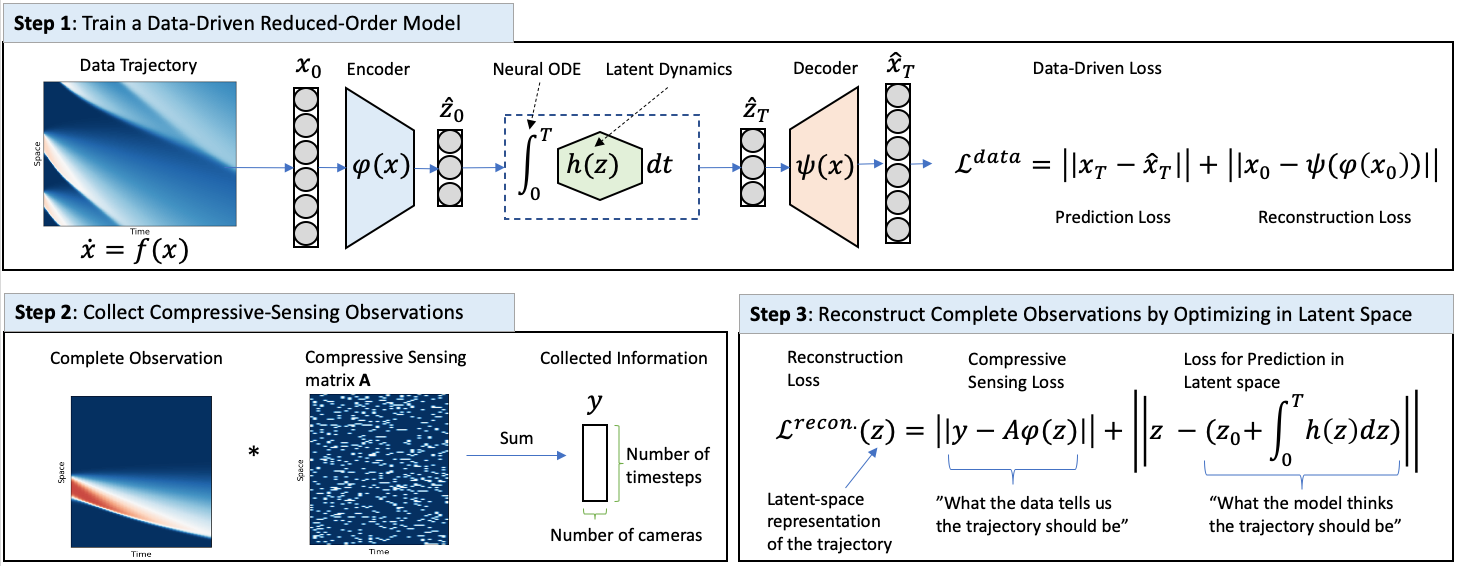
\includegraphics[width=\textwidth]{figures/cs_abstract.png}
    \caption{\label{fig:cs_abstract}We propose a compressive-sensing algorithm that reconstructs observations by identifying their trajectories in a latent space of a Reduced-Order Model (ROM). The model provides strong inductive bias and reduces data intake requirements for compressive-sensing hardware.}
\end{figure}

\paragraph{Reduced-Order Model with Non-Linear Latent Dynamics} We assume the same notation as in Section~\ref{sec:method} and define a reduced-order model (ROM) as a tuple $(\psi_\theta, \phi_\theta, h_\theta)$, which consists of a decoder $\psi_\theta(z)$, an encoder $\phi_\theta(z)$, and the latent dynamics $h(z)$, respectively, all parametrized by trainable weights $\theta$. We also assume that it is technically possible\footnote{For example, if $h(z)$ is a neural network, then one can evaluate such an integral using adjoint-sensitivity-based techniques, e.g. \texttt{torchdiffeq} package by \cite{chen2018neuralode}.} to evaluate a differentiable integral over the latent dynamics $h(z)$ for a given period of time. Figure~\ref{fig:cs_abstract} illustrates the architecture of the ROM. We assume that such ROM comes fully trained, so we consider its weights $\theta$ to be frozen and omit them from the notation. 

\paragraph{Compressive Sensing} In many applications, we can not observe $x(t)$ in real time. Instead, as illustrated on Figure~\ref{fig:cs_abstract} (Step 2), we observe $p$ scalar values per timeframe, with each scalar a linear combination of a small number of coordinates of $x(t)$ at a time:

\begin{equation}
    \label{eq:cs_definition}
    \tilde{y}(t) = A_t x(t), \quad A_t \in \mathbb{R}^{p\times n}
\end{equation}

When recorded over a discretized period of time $[t_1, \dots, t_T]$, such a set of observations is stored as a vector, $y \in \mathcal{R}^{T \times p} = [y(t_1), \dots, y(t_T)]^T$.

\begin{figure}
\centering
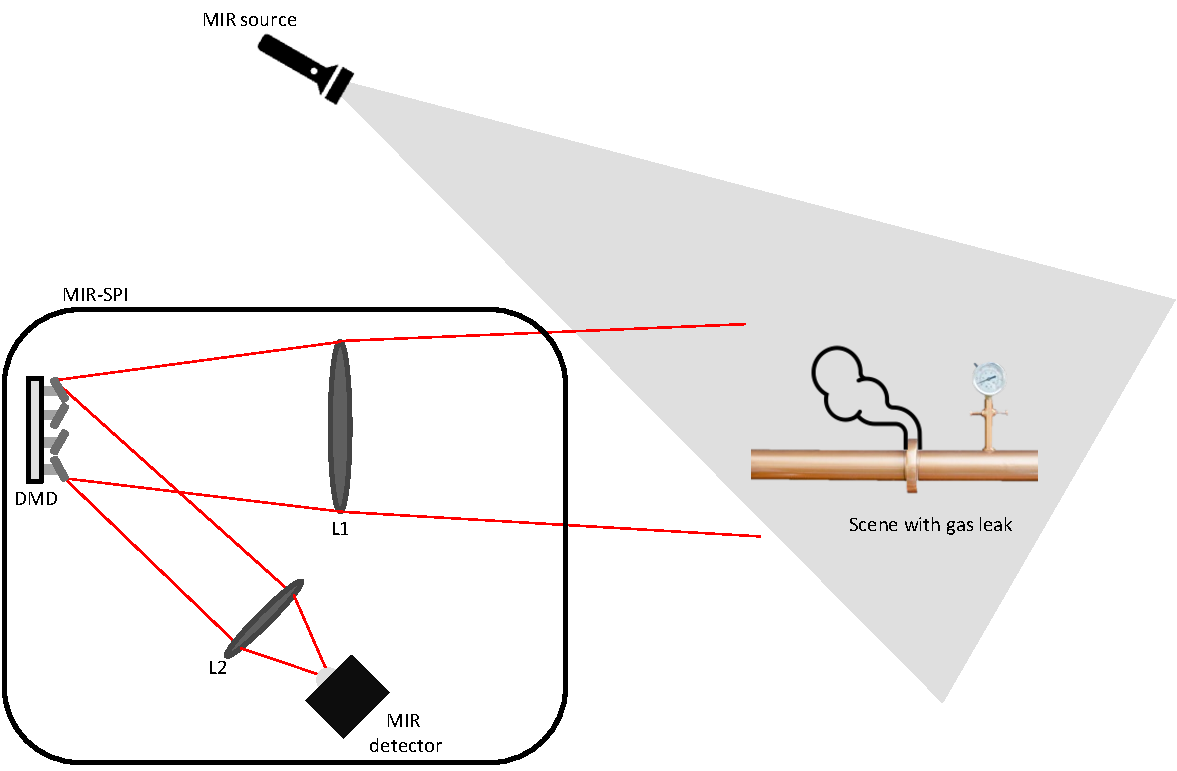
\includegraphics[width = 0.5\textwidth]{figures/SPI_setup.pdf}
\caption{SPI setup with DMD \label{fig:SPI}}
\end{figure}

We consider a single pixel camera setup in which, for every time instance $t$, $p$ acquisitions $y(t)$ are obtained by a high sampling rate photo-detector using the projection matrix $A_t$. The rows of the matrix $A_t$ correspond to a binary mask pattern that can be encoded using a digital micro-mirror device (DMD, \cite{pittman1995optical, sampsell1993overview}). Similarly to the setup from~\cite{duarte2008single}, the mirrors of our (idealized) DMD array represent pixels of the future reconstructed image, and the slopes of the mirrors represent the weights. The light from a scene lands on a DMD, which slopes each of its mirrors to reflect light either towards the detector (+1) or away from it (-1) according to a uniform Bernoulli variable. Next, the (+1) pixels go through a double-convex lens that focuses them on a signal photon detector. Finally, the detector integrates the signal and provides the final observation as its output voltage, which is later digitized by an A/D converter. The slopes of each mirror are also recorded in the detector's memory. Figure~\ref{fig:SPI} illustrates an example of the single pixel imaging setup where a gas plume is imaged using a DMD array and a medium infrared (MIR) photo-detector. 

A modern DMD supports snapshot frequencies of around 10~kHz (\cite{wang2022single}). When the scene changes much slower one can assume that such a device can take multiple measurements of a scene simultaneously\footnote{When the dynamics change rapidly, one would have to use an array of DMD devices to achieve more than one sample per frame}. The number of samples recorded per  frame is referred to as \textit{samples per frame}, or SPF. It is often divided by the total number of mirrors of the DMD device and multiplied by 100\%, in which case it is called a \textit{sample per frame rate} $\beta$. For a compressive-sensing-based image reconstruction approach to be practically useful it should require a relatively small rate $\beta$ (e.g. 2-10\%) for a successful reconstruction  of the scene.

\paragraph{Reconstruction Loss} It is often possible to have access to the complete state $x(t)$ at the moment of model training. Thus, one can develop a ROM $(\psi_\theta, \phi_\theta, h_\theta)$ using the full state $x(t)$, and then utilize this ROM for real-time compressive sensing applications. In particular, we use the ROM $(\psi_{\theta^*}, \phi_{\theta^*}, h_{\theta^*})$ from Figure~\ref{fig:cs_abstract}~(Frame 1) to forecast the dynamics based on partial observations in real time. Namely, instead of reconstructing $x(t)$ based on compressive-sensing observations $y(t)$ directly, we first reconstruct the latent dynamics $z(t)$ and then project it to the observable space using the decoder $\psi_{\theta^*}(z)$, as illustrated in Figure~\ref{fig:cs_abstract}, bottom-right pane. 

\begin{align}
    \label{eq:reconstruction_problem_differential}
    \min_{\{z_t\}_{t=1, \dots, T}} & \frac{1}{2}\sum_{t=1}^T \left\|y_t - A\psi_{\theta^*}(z_t)\right\|_2^2 \\
    \text{s.t. } & \dot{z} = h_{\theta^*}(z)
\end{align}

We integrate the constraint and write it in its Lagrangian form:
\begin{align}
\label{eq:reconstruction_problem_integral}
    \min_{\{z_t\}_{t=1, \dots, T}} \LL_{\theta^*}^{recon}(z)
\end{align}

where 

\begin{equation}
    \label{eq:reconstruction_loss}
     \LL_{\theta^*}^{recon}(z) = \frac{1}{2}\sum_{t=1}^T \left\|y_t - A\psi_{\theta^*}(z_t)\right\|_2^2 + \frac{\lambda}{2} \sum_{t=1}^T \left\|z_{t-1} + \int_{t-1}^{t}h_{\theta^*}(z)dz - z_t\right\|_2^2
\end{equation}

where the parameter $\lambda$ controls the degree on which the compressing sensing algorithm relies on the latent dynamics $h_{\theta^*}$ during the signal reconstruction phase. We minimize the loss~\eqref{eq:reconstruction_loss} using a gradient-based technique, with the gradients obtained using automatic differentiation frameworks. 

\subsection{Experiments}

\subsubsection{Burger's Equation}
We study the performance of our framework on Burger's equation with $[-\pi, \pi]$-periodic boundary conditions:

\begin{equation}
\begin{split}
    & u_t  + uu_x = \nu u_{xx} \\
    & u(-\pi, t) = u(\pi, t),\quad \forall t \in [0, T]
\end{split}
\end{equation}
where $u_t$, $u_x$, and $u_{xx}$ denote the first partial derivative in time, and the first and second spatial derivatives, respectively.

\paragraph{ROM Training} To obtain training data for the ROM, we replicate the experimental setup from Section~\ref{sec:compressibility}. Namely, we generate 1024 trajectories on a discretized spacial domain $[-\pi,\,\pi]$ with 128 grid points. To generate a diverse set of initial conditions, we sum the first 10 harmonic terms with random coefficients:
\begin{equation}
    \label{eq:burger_initial_condition_sine}
    u(x, 0) = \frac{1}{10}\sum_{k = 1}^{10} a_k\cos(kx) + b_k\sin((k+1)x), \quad a_k, b_k \sim \mathcal{N}(0, 1)
\end{equation}
 We solve Equation~\ref{eq:burgers_equation} for $t \in [0, 2]$ with $\Delta t = 0.1$ using a spectral solver by~\cite{trefethen2000spectral}. 

\paragraph{Compressive Sensing}
For the compressive sensing phase, we generate 128 trajectories with ``bump'' initial conditions -- a smooth approximation of a bump with two opposing steeply-curved sigmoids:

\begin{equation}
    \label{eq:burger_initial_condition_bumps}
    u(x, 0) = \frac{1}{1 + exp(-k(x-a))} - \frac{1}{1 + exp(-k(x-b))}
\end{equation}

where $a < b$ are sampled uniformly in $[-\pi, \pi]$ and $k = 20$. We choose this shape to ensure that the training and sensing trajectories are sufficiently different. We choose compressive sensing matrices $A_t$ to be binary (0-1) matrices with each row having 64 non-zero components out of 128 sampled uniformly.

We compare our approach (PINODE) with four alternatives: Digital Ghost Imaging (DGI) by~\cite{ferri2010differential} and~\cite{gong2010method}, its Autoencoder-enhanced variation (DGI+Conv. Decoder) by~\cite{wang2022single}, Total Variation Regularization  (TVR) by~\cite{bian2018experimental}, and an approach by~\cite{bora2017compressed} which uses an autoencoder (AE). We measure reconstruction accuracy with three commonly-used metrics: the residual mean-squared error (RMSE), the peak signal-to-noise ratio (PSNR), and the structural similarity index measure (SSIM). We evaluate both metrics for Burger's trajectories as 2D-images in spatial and in temporal domains. 

For two 2D images $a$ and $b$, PSNR is defined as the log-ratio of the maximal value from the true image:

\[
	\text{PSNR}(a, b) = 20\log\left(\frac{\max_{i,j}(|a[i,j]|)}{\|a - b\|_2}\right)
\]

SSIM is defined as a product of relative luminance $l(a,b)$, contrast $c(a,b)$, and structure $s(x,y)$:

\[
	\text{SSIM}(a, b) = l(a,b) \cdot c(a,b) \cdot s(a,b) = \left(\frac{2\mu_a\mu_b + c_1}{\mu_a^2 + \mu_b^2 + c_1}\right) \cdot \left(\frac{2\sigma_a\sigma_b + c_2}{\sigma_a^2 + \sigma_b^2 + c_2} \right) \cdot \left(\frac{\sigma_{ab} + c_2/2}{\sigma_a \sigma_b + c_2/2}\right)
\]
Finally, RMSE is defined as the mean residual squares for every state, averaged over the temporal axis:

\[
	\text{RMSE}(a,b) = \|a - b\|_F
\] 

where, for a picture $x$, $\mu_x$ is the pixel sample mean, $\sigma_x$ is the standard deviation,  and $c_i$ are the constants which stabilize the division when the denominator approaches 0. Typically, $c_i$ are set to be proportional to the square of the dynamic range of the pixel values, e.g.  $c_i = (k_i*2^{\text{bits per pixel}} - 1)^2$, with $k_1 = 0.01$ and $k_2 = 0.03$ being default choices.


\begin{figure}
    \centering
    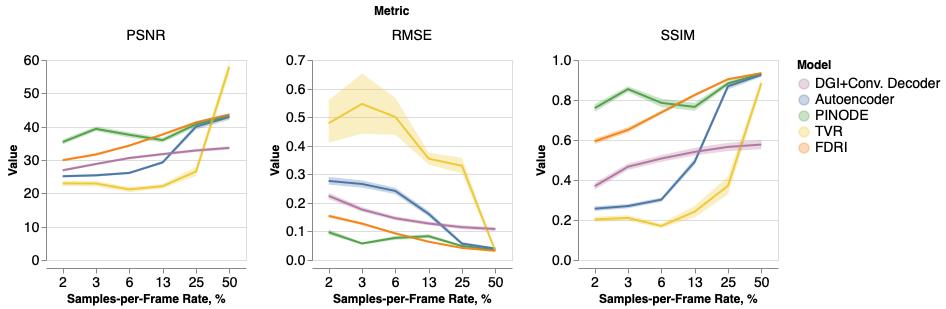
\includegraphics[width=\textwidth]{figures/cs_burgers_psnr.png}
    \caption{\label{fig:cs_burgers_spf} Median PSNR, RMSE, and SSIM with 25-27th percentile intervals over different number of samples per frame taken. We see that PINODE achieves 70\% higher peak signal-to-noise-ratio (PSNR), and 4 times higher structural similarity index measure (SSIM) when SPF is low, than its nearest competitor (AE).}
    
\end{figure}

\begin{figure}
    \centering
    	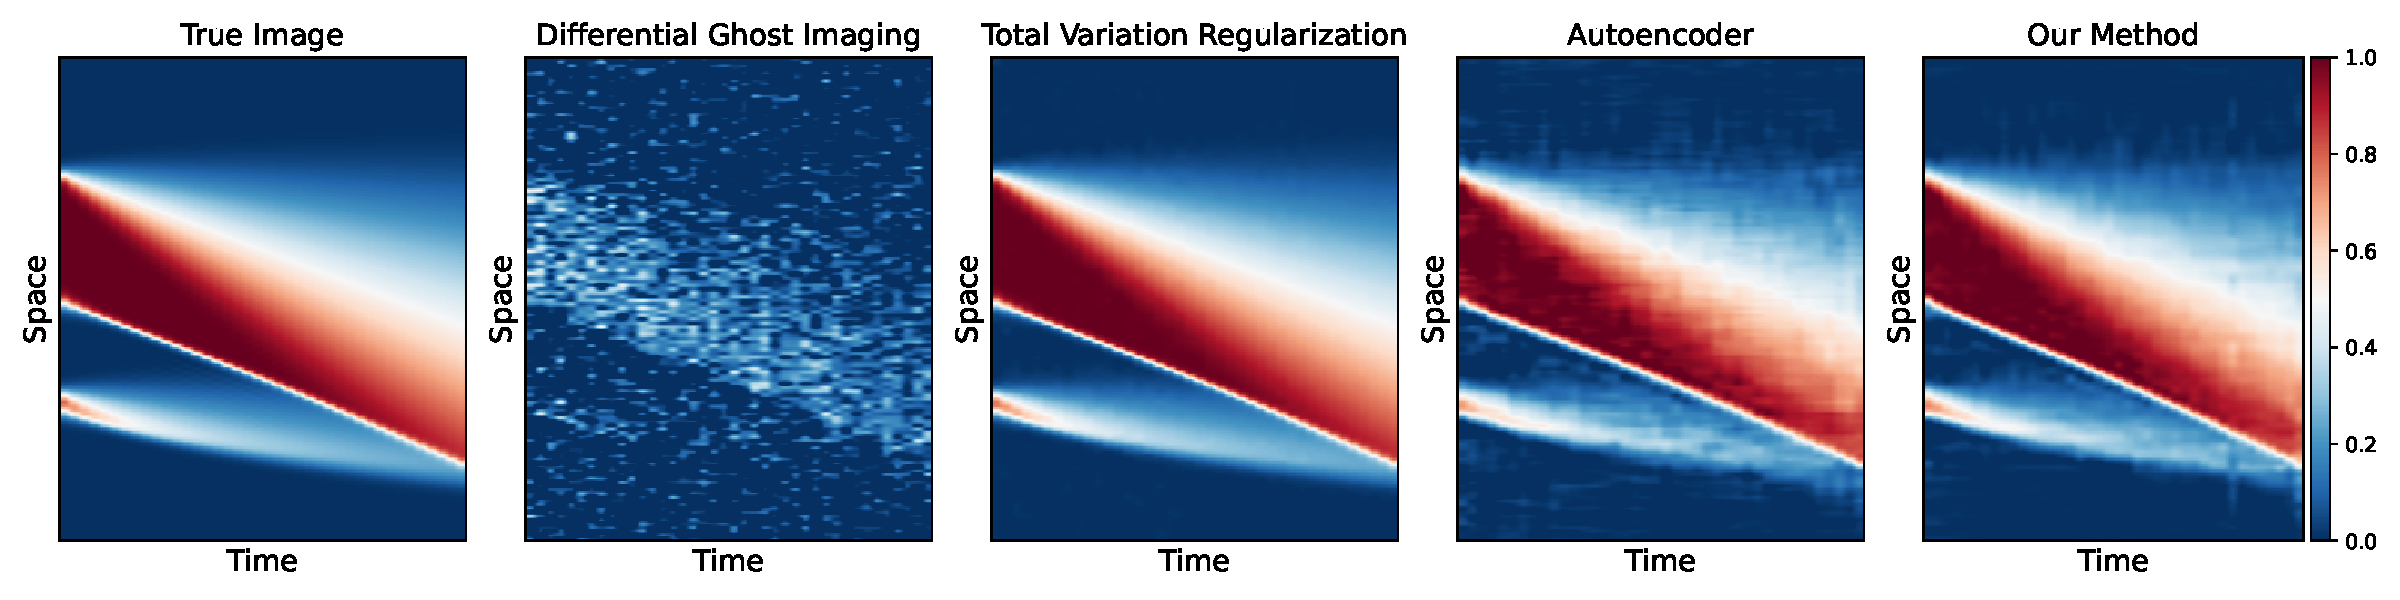
\includegraphics[width=\textwidth]{figures/cs_burgers_comparison_64.pdf}
    \caption{\label{fig:cs_burgers_example_large_spf} Example reconstruction with 32 samples per frame (SPF), an SPF rate of 50\%. Rather unsurprisingly, all algorithms complete the reconstruction faithfully due to a large amount of samples.}
\end{figure}

\begin{figure}
    \centering
    	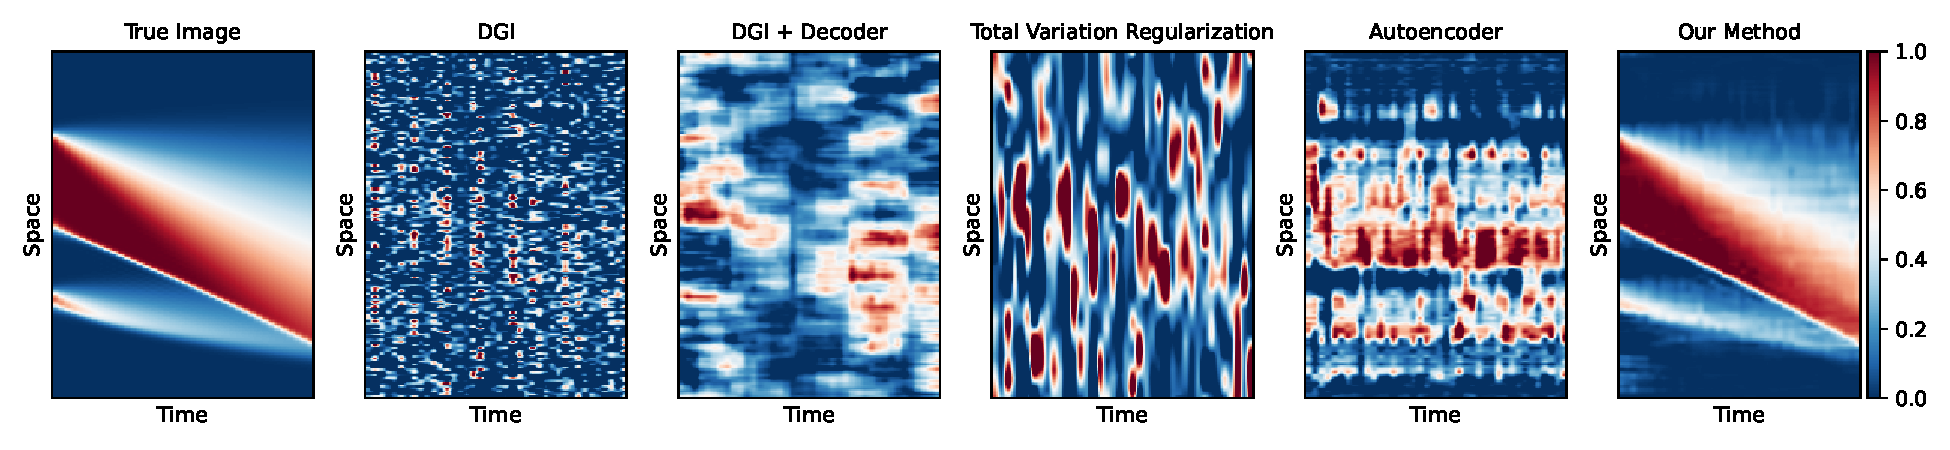
\includegraphics[width=\textwidth]{figures/cs_burgers_comparison_4.pdf}
    \caption{\label{fig:cs_burgers_example_small_spf}Example reconstruction with 2 samples per frame (SPF). All algorithms except our proposed method fail to recover the image due to the insufficient SPF rate (~3\%). In contrast, our proposed method achieves nearly the same reconstruction quality as in Figure~\ref{fig:cs_burgers_example_large_spf} with SPF rate of 50\%.}
\end{figure}

\paragraph{Results} The results are presented in Figure~\ref{fig:cs_burgers_spf}. We plot median PSNR, RMSE, and SSIM over different number of samples per frame taken. We see that PINODE achieves 70\% higher peak signal-to-noise-ratio (PSNR) and 4 times higher structural similarity index measure (SSIM)  relative other algorithms when SPF is low. We also see that the DGI and TVR approaches do not reconstruct images faithfully until SPF approaches the number of pixels in a snapshot; Figure~\ref{fig:cs_burgers_example_large_spf} provides an example of high-SPF reconstruction. In contrast, PINODE is able to reconstruct most trajectories with high accuracy using a very small number of samples per frame e.g. two samples, as visualized on Figure~\ref{fig:cs_burgers_example_small_spf}. It happens because the reduced-order model of PINODE serves as a strong prior: the model reconstructs the trajectory as a whole instead of reconstructing every snapshot separately, as all other algorithms do in this comparison. It allows PINODE to borrow strength across snapshots, even when SPF per each snapshot is small.

We also study robustness of PINODE approach to noise in compressive samples $y$ relatively to other algorithms. Figure~\ref{fig:cs_burgers_noise_aggregate} presents an aggregated comparison of reconstruction of solutions of Burger's equations under noise for SPF=12.5\%; the setup is equivalent to the one for SPF = 8 on Figure~\ref{fig:cs_burgers_spf} . Namely, we plot performance metrics (PSNR, RMSE, SSIM) of reconstructions from different models against Signal-to-Noise Ratio (SNR) in the vector of compressive sensing single-pixel observations $y$. The performance of PINODE remains superior until all models start reconstructing the scene very poorly. Figure~\ref{fig:cs_burgers_noise_examples} visualizes reconstructions for selected levels of SNR. We see that PINODE is able to provide a faithful reconstruction even under a substantial noise (e.g. third column).

\begin{figure}
	\centering
	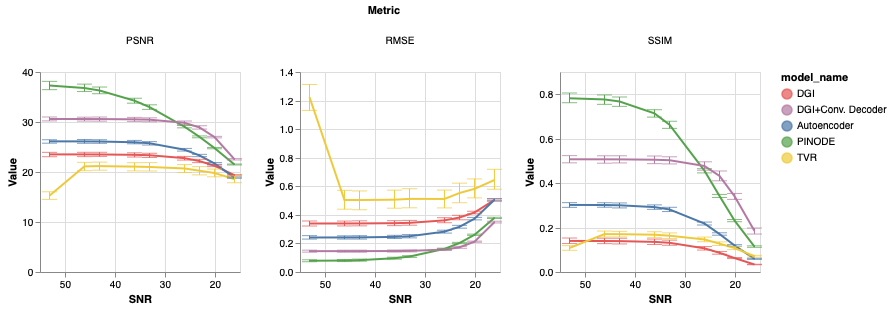
\includegraphics[width=\textwidth]{figures/cs_burgers_noise_aggregate.png}
	\caption{\label{fig:cs_burgers_noise_aggregate} Performance of reconstruction of solutions of Burger's equations under noise for SPF=12.5\%. We plot the performance metrics of different models against Signal-to-Noise Ratio (SNR) in the vector of compressive sensing single-pixel observations $y$. The performance of PINODE remains superior until all models start reconstructing the scene very poorly. See Figure~\ref{fig:cs_burgers_noise_examples} for example visualizations.}
\end{figure}

\begin{figure}
	\centering
	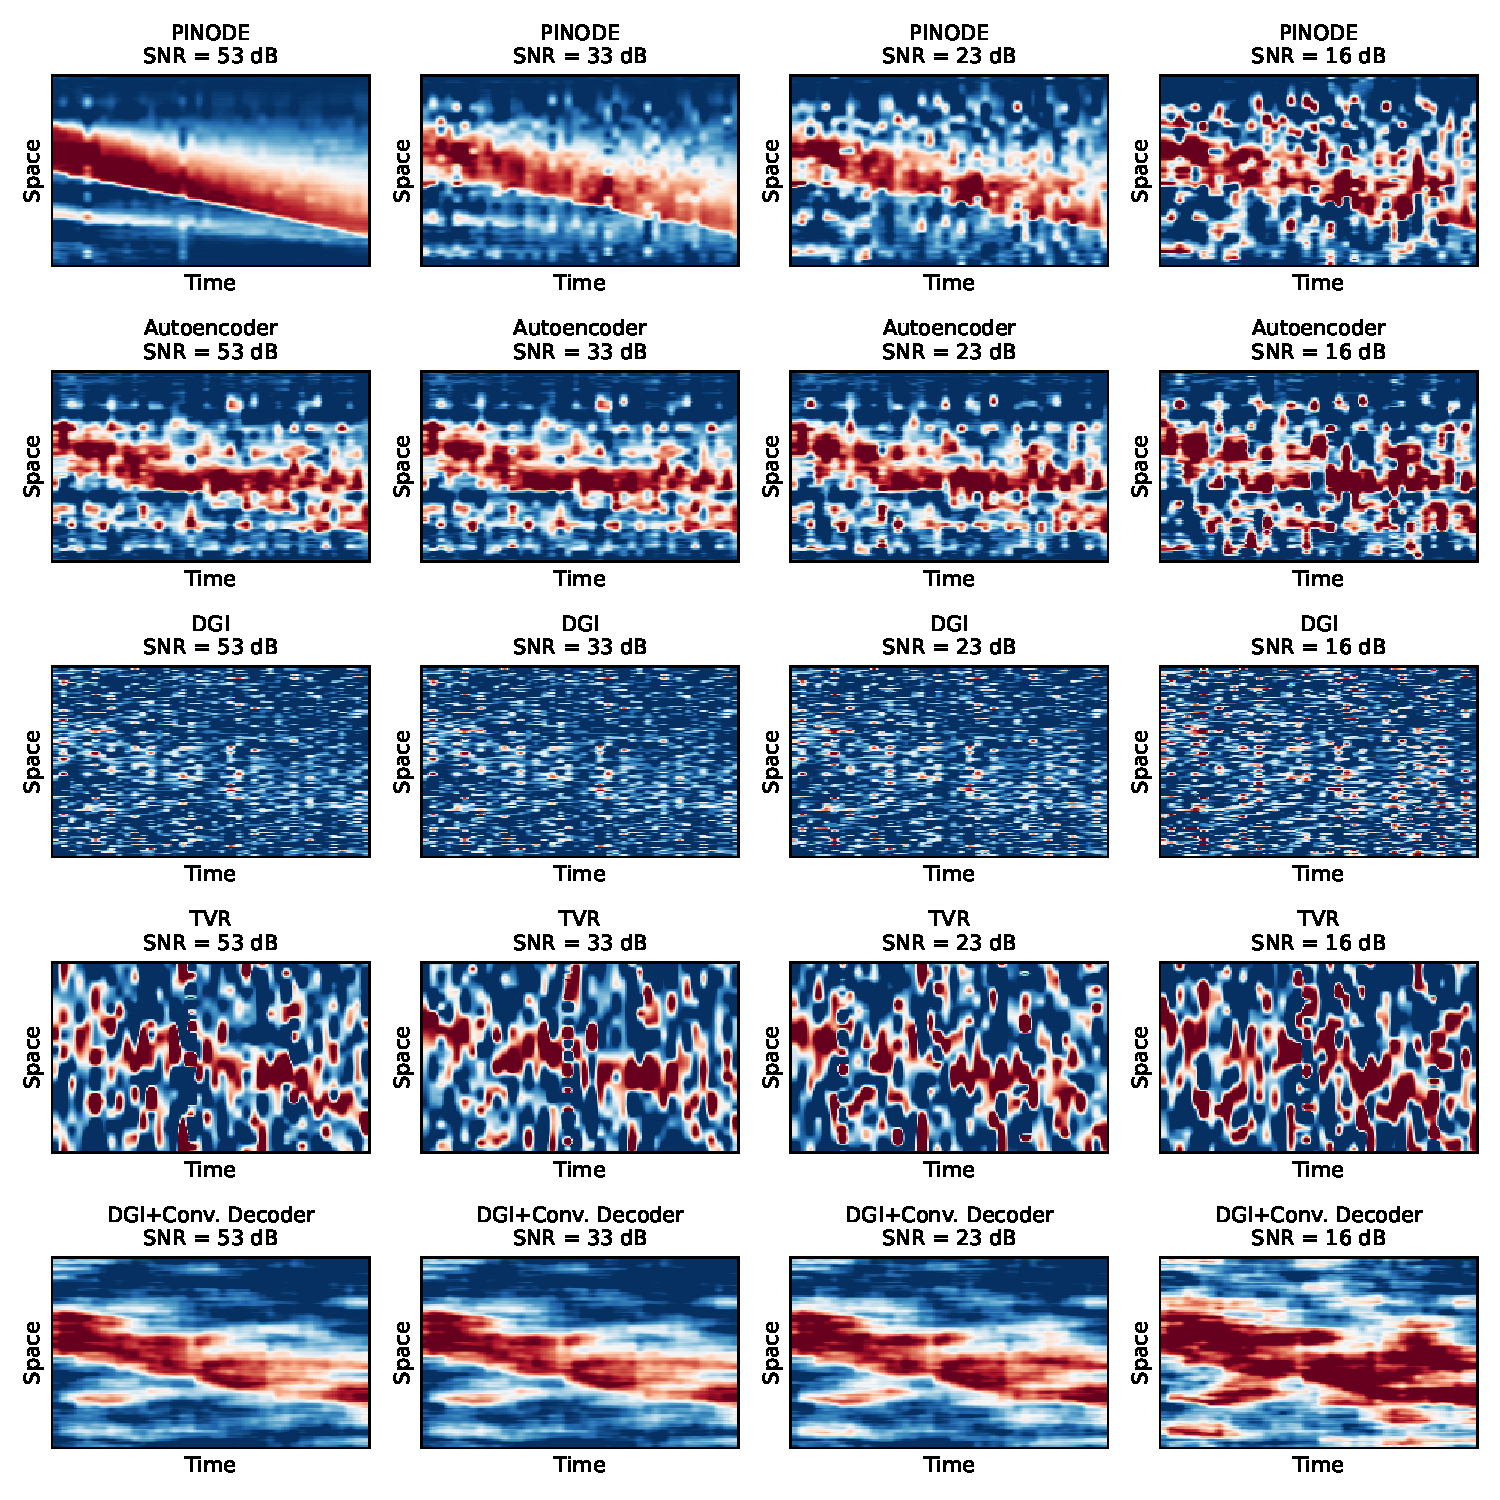
\includegraphics[width=\textwidth]{figures/cs_burgers_noise_examples.pdf}
	\caption{\label{fig:cs_burgers_noise_examples} Examples of compressive-sensing reconstructions of trajectories of Burger's equation under noise from Figure~\ref{fig:cs_burgers_noise_aggregate}.}
\end{figure}

 


\subsubsection{Kolmogorov Flow}
\label{sec:kolmogorov_flow}
We study the performance of our framework on Kolmogorov-like flow first-described by~\cite{dovzhenko1981generation} and later analyzed by \cite{tithof2017bifurcations,suri2017forecasting}. The following equation describes the behavior of a 2D velocity field $\bd{u}(x, y, t)$:


\begin{align}
\label{eq:kolmogorov_flow_definition}
	& \partial_t \bd{u} + \bd{u} \cdot \nabla \bd{u} = -\nabla p + \nu\nabla^2\bd{u} + f \\
	& \nabla \cdot \bd{u} = 0
\end{align}

where $p$ is a 2D pressure field, $f = \alpha\sin(ky)x$ represents the driving force with amplitude $A$ and wavenumber $k$, and $\nu = 1/\text{Re}$ is the non-dimensional viscosity equal to inverse of the Reynolds number. In all our experiments, $k = 4$ and $\text{Re} = 40$; we chose this setup to match the one from~\cite{wan2018data}, who identified that this combination of hyper-parameters leads to the occurrence of extreme instability events, making the prediction of such flow truly challenging. 

To train a ROM which predicts $u(x, y, t)$ we generate 8192 data trajectories as solutions of~\eqref{eq:kolmogorov_flow_definition} using a spectral solver\footnote{\href{https://github.com/zhong1wan/data-assisted/blob/master/Kolmogorov/kol2d_odd.py}{https://github.com/zhong1wan/data-assisted/blob/master/Kolmogorov/kol2d\_odd.py}} from~\cite{wan2018data}. Each solution was simulated from t=0 to t=100 to get past the transient regime and then recorded from t=100 to t=110, with the time-step $dt=0.5$. As in Section~\ref{sec:method}, the ROM consists of an encoder $\phi(u)$, a decoder $\psi(z)$, and the latent dynamics $h(z)$. It was trained by minimizing the data-driven loss~\eqref{eq:loss_data_driven} until the prediction RMSE on a holdout set stopped improving, which took about 60 epochs. 

\begin{figure}
	\centering
	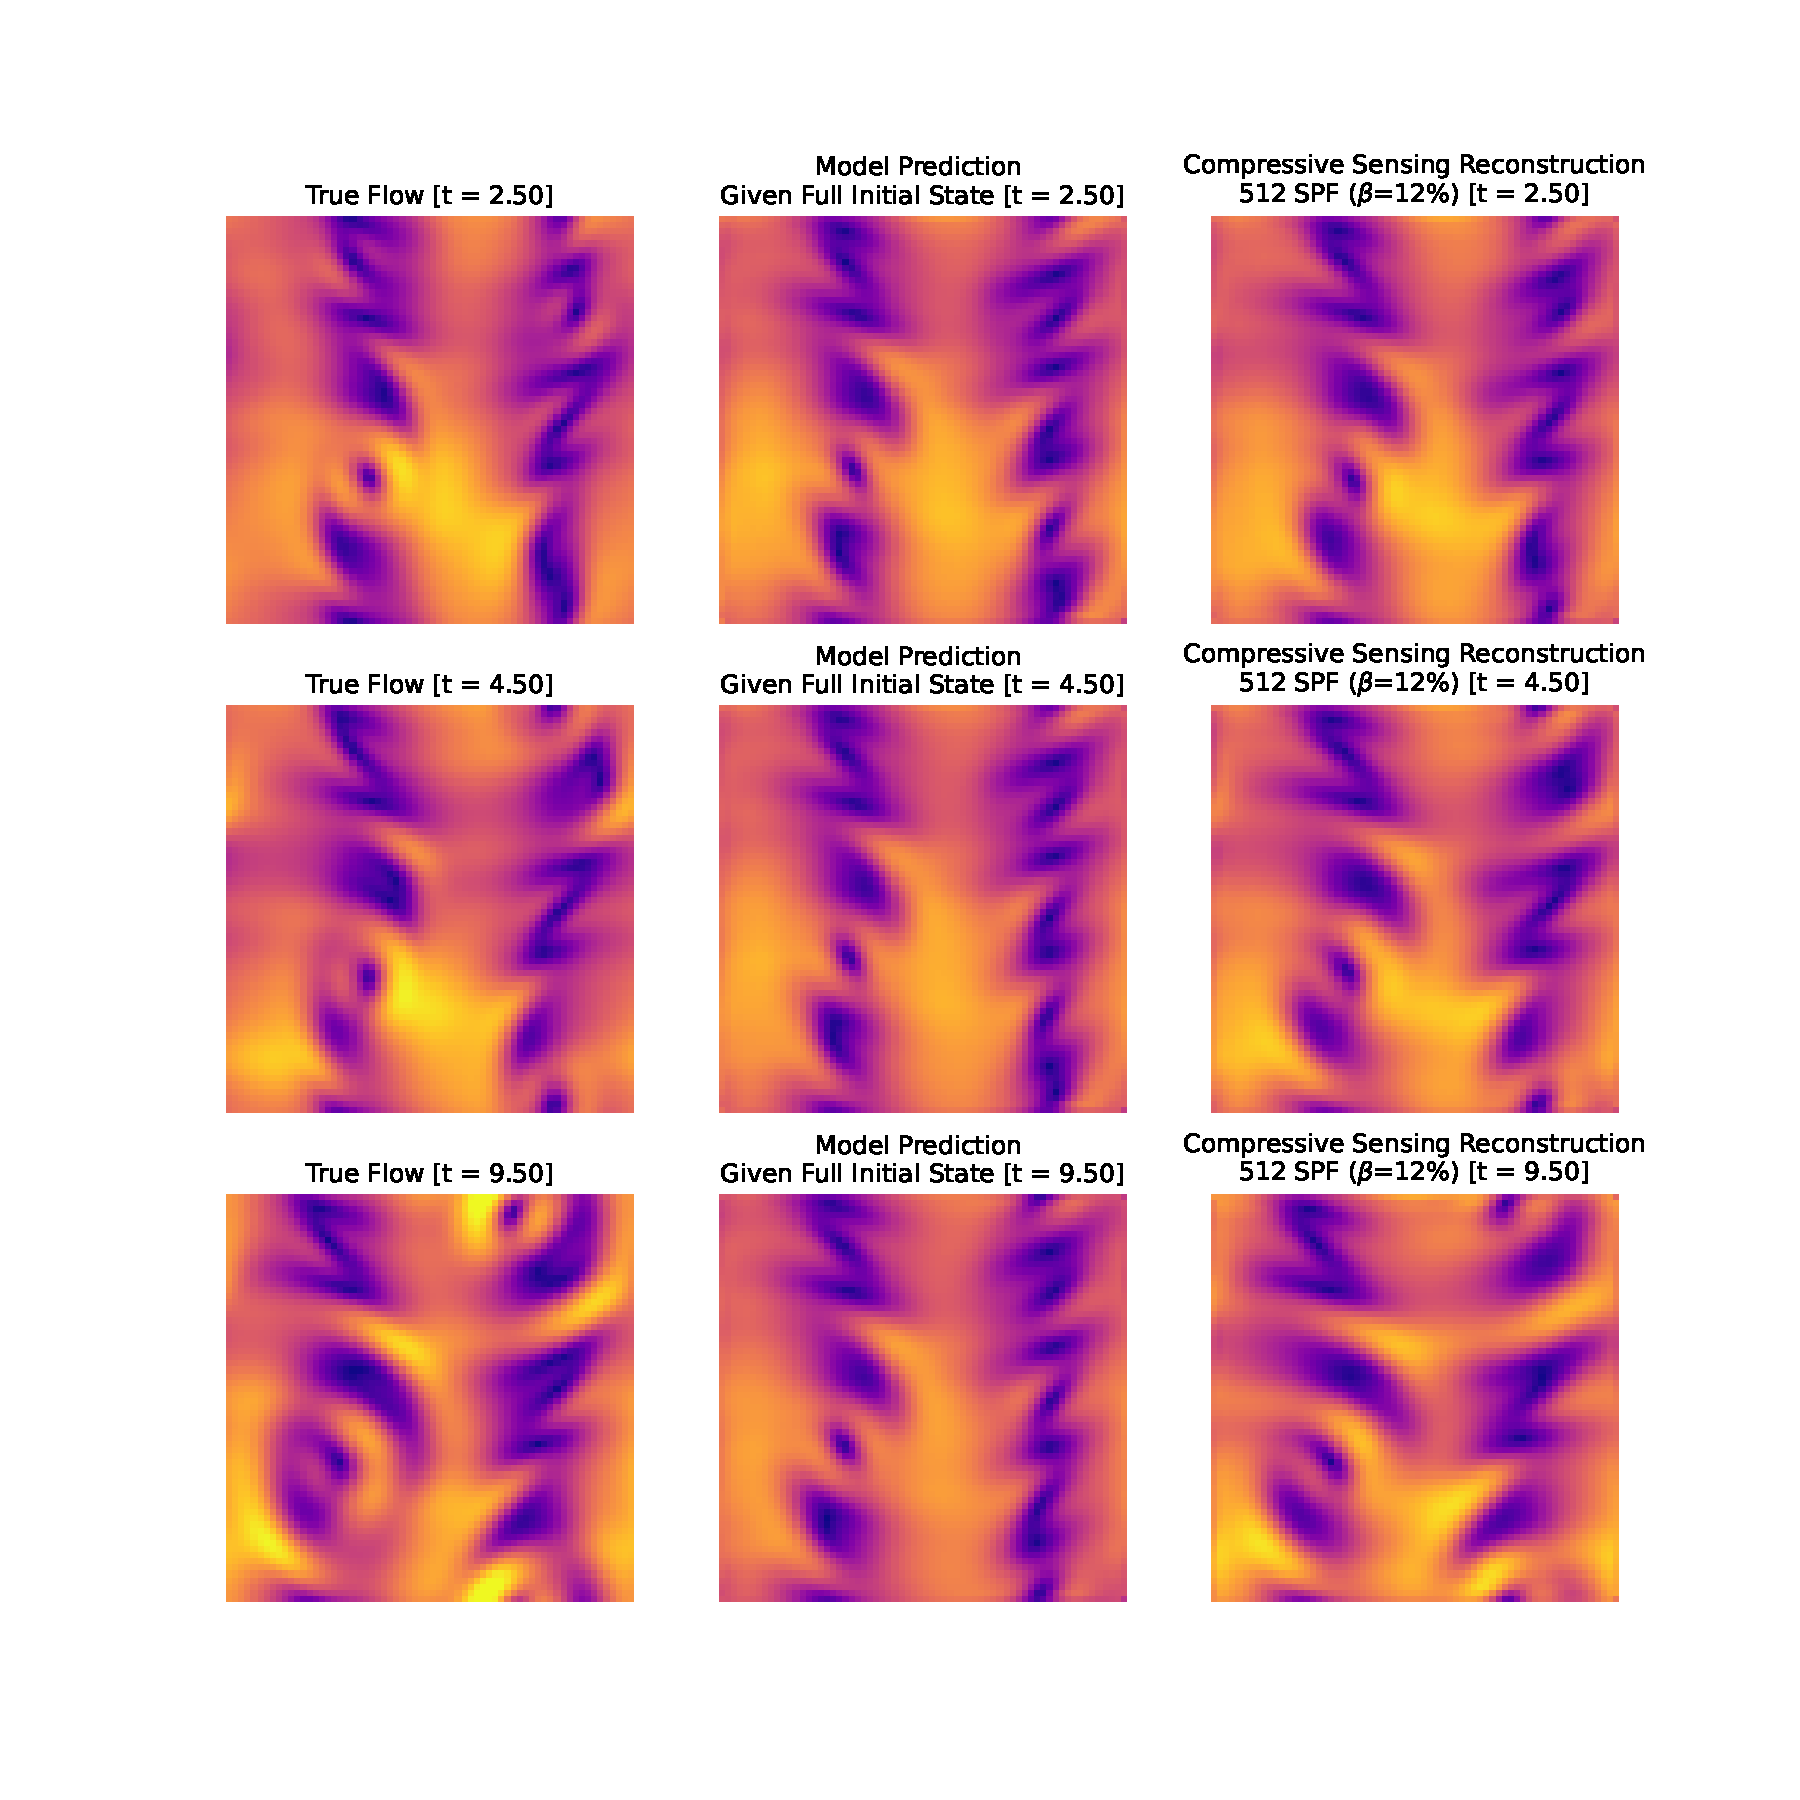
\includegraphics[width=\textwidth]{figures/kolmogorov_example.pdf}
	\caption{\label{fig:kolmogorov_example} An example of a compressive-sensing reconstruction of Kolmogorov flow using a ROM-regularized method. The rows represent three different moments in time. The first column represents the true flow. The second column represents a prediction of the ROM if the initial state of the system were to be known. The third column displays the results of CS reconstruction of our algorithm with 512 samples per frame.}
\end{figure}

A sample result is displayed on Figure~\ref{fig:kolmogorov_example}. The rows represent three different moments in time. The first column represents the true flow. The second column represents the prediction of the ROM if the initial state of the system were to be known to the model. It is unknown, so the second row serves as a reference performance of an underlying ROM. The third column displays the results of CS reconstruction of our algorithm with 512 samples per frame. Each frame is $66\times 66=4356$ pixels, which yields a sampling-per-frame rate of 12\%. We observe that the reconstruction faithfully recovered the signal. Moreover, we see that the CS algorithm is not limited in its performance by the performance of the underlying ROM: the third row indicates that the model is unable to completely recover shifting dynamics, whereas the CS algorithm aids the model's predictions with CS observations and fully reconstructs the signal.

\subsubsection{Methane Leaks Data}
In this section we use our technique to reconstruct videos of gas leaks using observations from a single-pixel camera. We use a subset of GasVid dataset by~\cite{wang2020machine} which consists of recordings of a methane gas leaks. 10 videos 10 to 20 seconds each. We split them into 1-second-long intervals, where each interval contains 10 steps: $T = 1$ sec., $dt = 0.1$ sec. Next, we remove backgrounds from each video using Gaussian Mixture-based Background/Foreground Segmentation (MOG2) algorithm by~\cite{zivkovic2006efficient,zivkovic2004improved} implemented in OpenCV library~(\cite{opencv_library}). Finally, we split all intervals into four non-overlapping batches: train (390), dev (50), test (49), and compressive sensing (2). We use the first three to train, fine-tune, and select a final ROM respectively, and then we use the fourth batch for compressive sensing reconstruction. We use the same architecture of ROM as in Section~\ref{sec:kolmogorov_flow}. At the compressive sensing step we sample 512 single-pixel observations per each $240 \times 320$ video frame; it corresponds to SPF ratio of $0.66\%$ (2/3 of one percent).

\begin{figure}
	\centering
	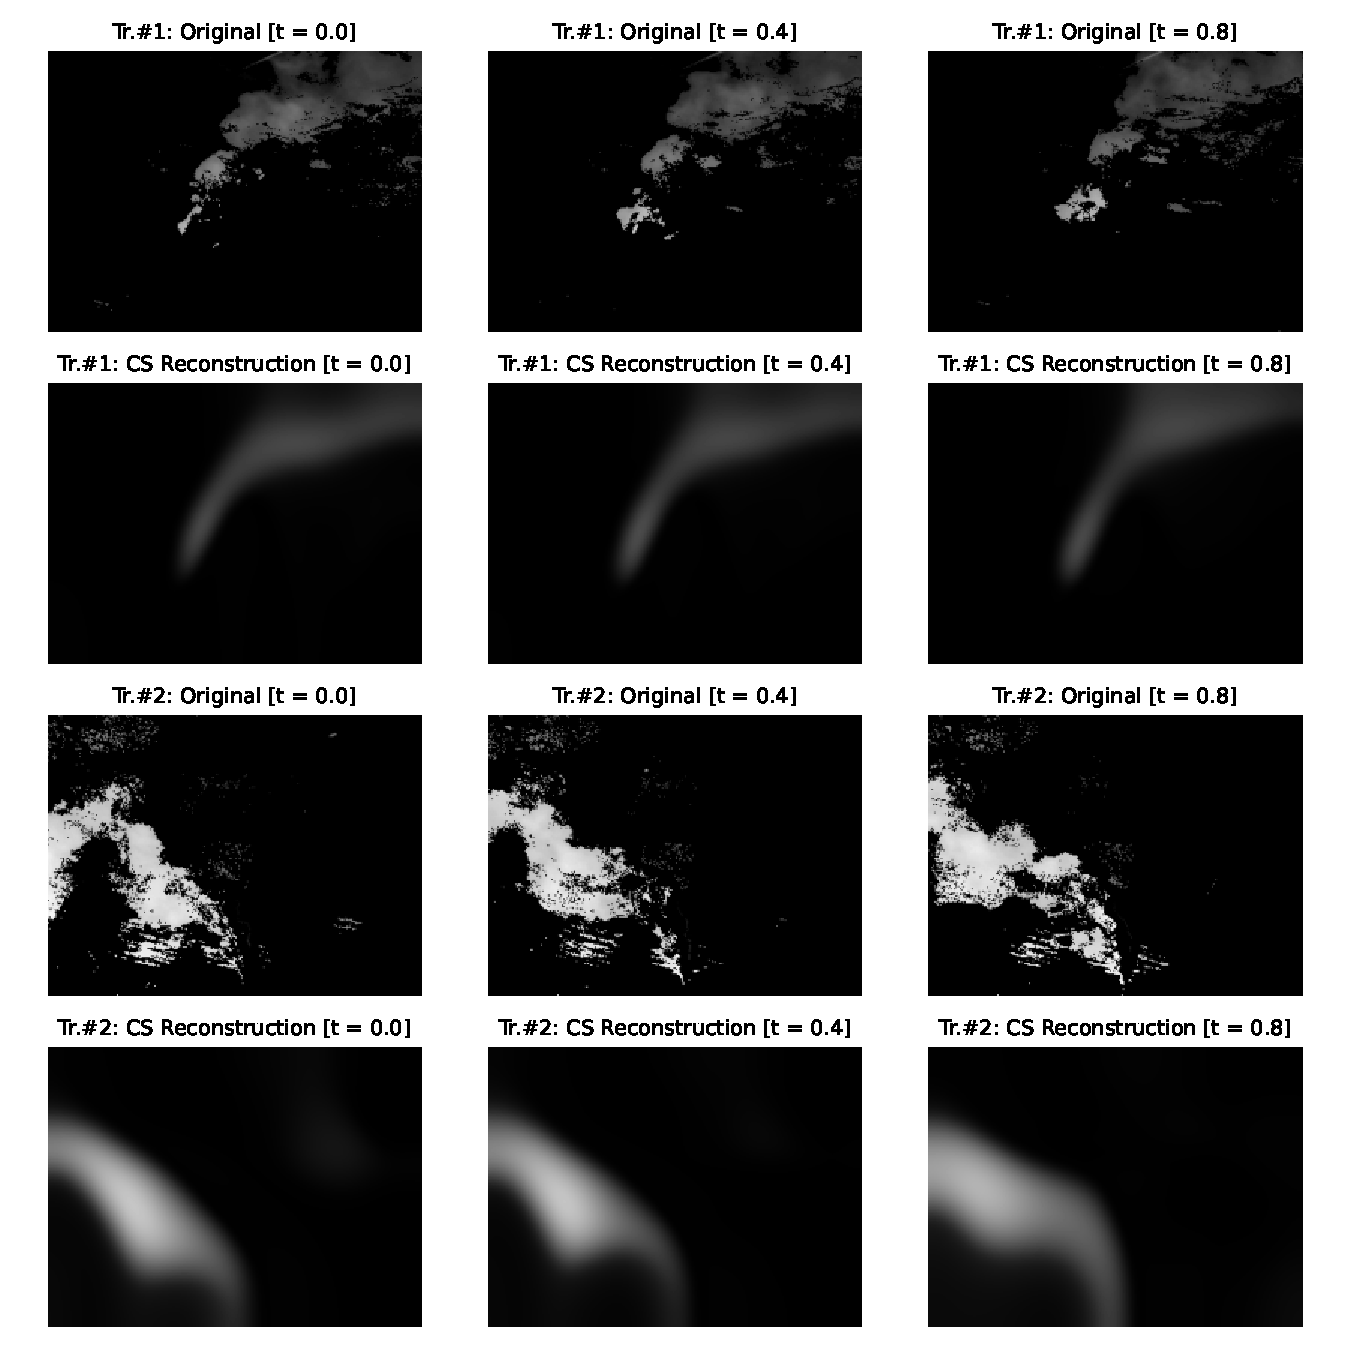
\includegraphics[width=\textwidth]{figures/cs_gas_examples.pdf}
	\caption{\label{fig:cs_gas_examples}}
\end{figure}

The example reconstructions are presented on Figure~\ref{fig:cs_gas_examples}. We see that the algorithm was able to faithfully reconstruct the trajectories. Although it was unable to capture the details of turbulent flows, it was able to predict the altitude, the direction, and the spread of the plumes correctly, which are the most important aspects for practical applications in real-world gas monitoring applications. 

We note the threefold difficulty of the task. First, the background subtraction struggles to separate grey smoke from a dynamic grey background, which leads to fantom clouds of smoke in processed data. Second, the amount of training data (3900 frames) is extremely small for training a large convolutional ROM. For example, \cite{wang2020machine} used the same dataset for training a simpler classification network (leak/non-leak) using ~11000 frames. Finally, an SPF of 0.66\% is vastly insufficient for frame-by-frame reconstruction, as most state-of-the-art methods require ~5-10\% SPF, depending on the nature of the picture (	\cite{wang2022single}). Thus, the inductive bias of the ROM becomes a crucial component for a successful video reconstruction.


\subsection{Discussion} 
In this work, we demonstrated how a collocation-point-based technique can improve the performance of an emerging class of continuous-time physics-informed neural-network-based reduced-order models. First, we demonstrated that the incorporation of collocation points in training data can ``cover the gaps'' in training trajectories and inform the model about underrepresented basins of attraction. Such an approach alleviates the demand for large volumes of data that is common in network-based models. Reducing the amount of data required to faithfully reconstruct a signal is extremely valuable in applications where data is scarce and expensive. Second, the physics-informed loss may work as a safeguard, providing a noise-free source of underlying dynamics.
Third, collocation points can stabilize the model's long-term predictions, allowing for accurate forecasting far beyond the training time horizon. Finally, together with using neural-ODE-based nonlinear latent dynamics, adding physics-informed loss leads to the discovery of more compact latent space representations that also yield more accurate models. Simultaneous stability and compactness is especially important if one aims to use models with compressive sensing and control algorithms. With respect to the computational complexity, we note that adding $Tk$ collocation points to the training imposes less of a computational burden than adding $k$ data trajectories, because, unlike data trajectories, collocation points do not require computing integrals forward in time. The last section served to illustrate how PINODE models that were developed in Section~\ref{sec:method} can help in applied modeling. In particular, we showed how one can employ a PINODE model for compressive-sensing purposes. We illustrated its performance on two examples: Burger's equation and Kolmogorov flow. In these cases, it is clear that PINODE can serve as a powerful regularizer and allow users to go significantly below the limits of the Nyquist sampling theorem. 

One clear limitation of the current work is that the choice of an efficient collocation family is a design decision that a practitioner makes. We believe that such decisions can be automated by adopting existing approaches from classic works on numerical approximations of PDEs, which we leave for future research. Another automation that prompts future research is deriving efficient ways of sampling collocation points, possibly via applying modern adaptive learning techniques \cite{subramanian2022adaptive}. Finally, although Section~\ref{sec:burger_noise} provides some rationale for why one may expect robustness of hybrid models under noise, we believe that a more rigorous analysis is possible, particularly one that provides conditions under which such robustness is guaranteed. 
